\documentclass[review]{elsarticle}

\usepackage{lineno,hyperref}

%extras
\usepackage{eurosym}
\usepackage{graphicx}
\usepackage{cleveref}
\usepackage{pdflscape}
\usepackage{color}

\usepackage{longtable}
\usepackage{url}
\newcommand{\TG}[1]{\color{red}\textbf{Tristan:} #1
\color{black}}

\modulolinenumbers[5]

\newcommand{\changedtext}[1]{
	\textcolor{red}{\textbf{#1}}
}


\journal{FGCS, Special Issue on Science Gateways, 2018}


%%%%% TODO
% correct bib
% -- harmonize usage of et al
% -- references to urls 
% -- references to complete proceedings

%%%%%%%%%%%%%%%%%%%%%%%
%% Elsevier bibliography styles
%%%%%%%%%%%%%%%%%%%%%%%
%% To change the style, put a % in front of the second line of the current style and
%% remove the % from the second line of the style you would like to use.
%%%%%%%%%%%%%%%%%%%%%%%

%% Numbered
\bibliographystyle{model1-num-names}

%% Numbered without titles
%\bibliographystyle{model1a-num-names}

%% Harvard
%\bibliographystyle{model2-names.bst}\biboptions{authoryear}

%% Vancouver numbered
%\usepackage{numcompress}\bibliographystyle{model3-num-names}

%% Vancouver name/year
%\usepackage{numcompress}\bibliographystyle{model4-names}\biboptions{authoryear}

%% APA style
%\bibliographystyle{model5-names}\biboptions{authoryear}

%% AMA style
%\usepackage{numcompress}\bibliographystyle{model6-num-names}

%% `Elsevier LaTeX' style
%\bibliographystyle{elsarticle-num}
%%%%%%%%%%%%%%%%%%%%%%%

\begin{document}

\begin{frontmatter}

\title{The Global Impact of Science Gateways, Virtual Research Environments and Virtual Laboratories}


\author[michele]{Michelle Barker\corref{mycorrespondingauthor}}
\cortext[mycorrespondingauthor]{Corresponding author}
\address[michele]{ 
	National eResearch Collaboration Tools and Resources and James Cook University, Australia}
\ead{michelle.barker@nectar.org.au}

\author[silvia]{Silvia Delgado Olabarriaga}
\address[silvia]{
	Amsterdam Medical Centers -- Location AMC, University of Amsterdam, The Netherlands
}

\author[nancy]{Nancy Wilkins-Diehr}
\address[nancy]{
	San Diego Supercomputer Center, University of California San Diego, USA
}

\author[sandra]{Sandra Gesing}
\address[sandra]{
Department of Computer Science and Engineering/Center for Research Computing, University of Notre Dame, USA}
%orcid.org/0000-0002-6051-0673

\author[dan]{Daniel S. Katz}
\address[dan]{National Center for Supercomputing Applications, Department of Computer Science, Department of Electrical and Computer Engineering, School of Information Sciences, University of Illinois at Urbana-Champaign, USA}
%  d.katz@ieee.org http://orcid.org/0000-0001-5934-7525

\author[shayan]{Shayan Shahand} 
\address[shayan]{ServiceNow and Academic Medical Center -- University of Amsterdam, The Netherlands}

\author[scott]{Scott Henwood}
\address[scott]{CANARIE, Canada}

\author[tristan]{Tristan Glatard} 
\address[tristan]{Department of Computer Science and Software Engineering, Concordia University, Canada}


\author[keith]{Keith Jeffery}
\address[keith]{VRE4EIC and ERCIM, UK}

\author[brian]{Brian Corrie} 
\address[brian]{Simon Fraser University, Canada and New Zealand eScience Infrastructure, New Zealand}
%orcid.org/0000-0003-3888-6495

\author[andrew]{Andrew Treloar}
\address[andrew]{Australian National Data Service, Australia}
%orcid.org/0000-0002-8911-3081

\author[helen]{Helen Glaves} 
\address[helen]{British Geological Survey, UK}
%orcid.org/0000-0001-8179-4444

\author[lesley]{Lesley Wyborn}
\address[lesley]{National Computational Infrastructure Facility and The Research School of Earth Sciences, Australian National University, Australia}
%http://orcid.org/0000-0001-5976-4943

\author[neil]{Neil P. Chue Hong} 
\address[neil]{University of Edinburgh, UK}
%http://orcid.org/0000-0002-8876-7606

\author[alex]{Alessandro Costa}
\address[alex]{INAF, Italy}
%https://orcid.org/0000-0003-0344-8911



\begin{abstract}
Science gateways, virtual laboratories and virtual research environments are all terms used to refer to community-developed digital environments that are designed to meet a set of needs for a research community. Specifically, they refer to integrated access to research community resources including software, data, collaboration tools, workflows, instrumentation and high-performance computing, usually via Web and mobile applications. Science gateways, virtual laboratories and virtual research environments are enabling significant contributions to many research domains, facilitating more efficient, open, reproducible research in bold new ways. 
This paper explores the global 
\changedtext{impact achieved by the sum effects} of these programs in increasing research impact, demonstrates their value in the broader digital landscape and discusses future opportunities. 
\changedtext{This is evidenced through examination of national and international programs in this field.}
\end{abstract}

\begin{keyword}
science gateways \sep virtual research environments \sep virtual laboratories \sep open science \sep e-infrastructure \sep cyberinfrastructure
\end{keyword}

\end{frontmatter}

\linenumbers

\section{Introduction}
%\nocite{*}

Science gateways, virtual laboratories and virtual research environments (hereafter science gateways) refer to various kinds of community-developed digital interfaces to advanced technologies that support research. 
They are used in a wide variety of scientific domains, from high-energy physics and astrophysics to humanities and the social sciences. By tailoring digital environments to community needs, science gateways perform a key role in integrating elements of the e-infrastructure landscape, providing online access to software, data, collaboration tools, instrumentation and high-performance computing, to facilitate increased research impacts.

Science gateways are enabling significant contributions in many research domains, with national and international initiatives to develop gateways further demonstrating their importance and value. 
This paper explores the global impact of these programs, highlighting their successes, value in the broader landscape and future focus. 
\changedtext{The paper begins with a discussion on the definition of terms, then documents national and international programs in this field to illustrate the global impact achieved by  the sum effects of these  initiatives.}
This investigation then highlights the role and value of science gateways in the digital research environment, and examines the impact of science gateways, to evidence how science gateways facilitate more efficient, open, reproducible research in bold new ways. 
A discussion of challenges and opportunities ahead concludes the study. 

\section{Definition of terms}

A number of terms are often used in this field, including science gateways, virtual laboratories and virtual research environments (VREs). Different terms exist in large part for historical reasons; science gateways evolved in the USA, virtual laboratories in Australia, and VREs in Europe. 

Shahand's analysis of science gateways research defines science gateways as ``web-based enterprise information systems that provide scientists with customized and easy access to community-specific data collections, computational tools and collaborative services on e-Infrastructures.''~\cite{shahand2015-1} This definition is similar to that used by the Science Gateways Community Institute, the USA's National Science Foundation-funded coordination project in this area, which also differentiates between science gateways and the generic cyberinfrastructure on which they build~\cite{what-is-sg-2}. Australia's virtual laboratory community uses similar definitions, with an emphasis on access to integrated data, computational environments and tools~\cite{nectar-impact-3}. 

Between 2004--2011, Jisc funded the development of a number of VREs in the UK, and defined VREs more broadly than science gateways and virtual laboratories: ``The term VRE is now best thought of as shorthand for the tools and technologies needed by researchers to do their research, interact with other researchers ... and to make use of resources and technical infrastructures available both locally and nationally.''~\cite{jisc-vre-4} Horizon 2020, the European Commission's research and innovation framework programme, suggests that VREs ``should integrate resources across all layers of the e-infrastructure (networking, computing, data, software, user interfaces), should foster cross-disciplinary data interoperability and should provide functions allowing data citation and promoting data sharing and trust.''~\cite{h2020-vre-5} 

Carusi and Reimer's work notes the relevance of alternative terms including collaborative e-research community, collaboratory and virtual research community~\cite{,Carusi2010-6} and identifies convergence on a set of characteristic features: ``an electronic web-based environment for a) access to data, tools, resources; b) co-operation or collaboration with other researchers; c) cooperation at the intra- and inter-institutional levels; or d) preserving or taking care of data and other outputs.'' 
Candela, Castelli and Pagano's analysis of VREs also identifies five distinguishing features that are similar, however focussed on communities of practice~\cite{candela2013-7}. 
\changedtext{A community of practice is a group of people who share some expertise in a specific field or common interest, and who learn from each other through information sharing~\cite{lave-wenger-1991}. The distinguishing features are: }
 ``(i) it is a web-based working environment;  (ii) it is tailored to serve the needs of a community of practice;  (iii) it is expected to provide a community of practice with the whole array of commodities needed to accomplish the community's goal(s); (iv) it is open and flexible with respect to the overall service offering and lifetime; and (v) it promotes fine-grained controlled sharing of both intermediate and final research results by guaranteeing ownership, provenance and attribution.''  
 Shahand also suggests that science gateways usually have five functional properties: usability, scalability, integration, automation and sharing and reuse~\cite{shahand2015-1}. 

It should be noted that science gateways can vary in scope depending on the problems they aim to address and the domains they support. In this paper, an inclusive definition of science gateways is used, covering all the aspects raised above.

\section{Science gateways activities around the globe}

Activities involving science gateways are growing around the globe, with the establishment of programs, organizations, conferences and special issues in scientific journals.
\changedtext{These are collectively facilitating more efficient, open, and reproducible research worldwide.}

\subsection{Programs and Organizations}

Whilst science gateways have historically been enabled through a wide variety of mechanisms, they are now increasingly facilitated through national and international programs that specifically facilitate their development and sustainability. 
National and international programs focusing on the development of science gateways include:

\begin{itemize}

\item \emph{CANARIE}, a non-profit corporation, with the major investment in its programs and activities provided by the Government of Canada, funds the development of research software that enables Canadian researchers to more quickly and easily access research data, tools and collaborators. Since 2007, CANARIE has provided funding for 37 science gateway projects in disciplines such as high energy physics, astronomy, astrophysics, oceanography, human kinetics, robotics, bioinformatics, genomics, neurology, cartography, immunology, mechanical engineering, civil engineering, Arctic research, video analysis, animal biology, digital humanities, climatology, forestry, road traffic management, and e-Health~\cite{canarie-15}. 

\item Science Gateways Community Institute (\emph{SGCI}), funded in 2016 for \mbox{USD\$15 million} by USA's National Science Foundation (NSF) to act as a focal point to facilitate the development of a sustainable software ecosystem for science gateways~\cite{sgci-16}.
\changedtext{The institute has funding for 2016-2021, with an  opportunity to retain funding for an additional 5 years.}
 SGCI's programs include a business incubator, extended developer support, scientific software collaborative, community engagement and exchange and workforce development. It is one of the two initial Scientific Software Innovation Institutes funded under NSF's Software Infrastructure for Sustained Innovation (SI2) program~\cite{nsf-si-17}. SI2 funds software projects of varying scales, from small research software groups to the large software institutes, including specific science gateways themselves as well as projects developing general software that can be used to build gateways. 

\item European Comission (\emph{EC}) funding programs for research and innovation include the Seventh Programme Framework (\emph{FP7}) and \emph{Horizon 2020}. FP7 supported VRE projects from 2007-2013.
For example, SCI-BUS explored new possibilities for European user communities to create custom science gateways through a generic-purpose gateway technology~\cite{kacsuk2014-18}. 
The project created a toolset to provide seamless access to major computing, data and networking infrastructures and services in Europe, including clusters, supercomputers, grids, desktop grids, academic and commercial clouds. Similarly, the Catania Science Gateway Framework~\cite{decide-19} and its successor FutureGateways~\cite{futuregateway} provide application developers with tools to develop science gateways quickly and easily. 
Since 2014, Horizon 2020 has supported a number of European VRE projects including BlueBridge, EVER-EST, VRE4EIC, WEST-Life, VI-SEEM and MUG~\cite{h2020-projects-20}. 
Most VREs are domain-specific, however there are also now initiatives creating toolsets for the creation of science gateways. 
For example, VRE4EIC, a Horizon 2020 research project totaling \euro 4.37 million over 3 years, will provide a VRE reference model, a set of VRE components and a prototype Europe-wide interoperable VRE to empower multidisciplinary research communities~\cite{vre4eic-21}. 
Other Horizon 2020 projects include Sci-GalA (Energizing Scientific Endeavour through Science Gateways and meta-Infrastructures in Africa), a \euro 1.4 million project that promotes the uptake of science gateways and strengthens and expands supporting e-infrastructures in Africa and beyond~\cite{sci-gaia-22}.

\item National eResearch Collaboration Tools and Resources (\emph{Nectar}), funded by the Australian Government \changedtext{(2011-2017)}, has distributed over AUD\$20 million since 2011 specifically to facilitate software infrastructure programs that included the development of fourteen virtual laboratories. These virtual laboratories have received an additional AUD\$20 million in co-investment~\cite{nectar-impact-3}. By 2018, the virtual laboratories recorded over 23,000 users, and on average each virtual laboratory included users from over 20 international and 30 Australian organizations.

\end{itemize}

\changedtext{Note that these programs are very diverse in organization and level of funding. This hampers their comparison, so the examples above should be taken as illustrations rather than a complete and systematic overview.
In addition to these coordinated programs, there are also many gateways being developed and sustained with direct funding through their own research grants. Although it is difficult at the moment to estimate the actual budgets of these initiatives, the 400+ entries in the SGCI gateway catalog\cite{sgci-16} (400+) can serve as an indication of the impressive amount of investments taking place in this way.}

\subsection{Collaborative Initiatives}

A common observation in these national and international programs is that the development of science gateways is increasingly complex, therefore communities of practice have formed across international initiatives through global consortia. The very impetus for this paper comes from the \emph{International Coalition on Science Gateways}, an international forum that brings together national, regional and international initiatives to provide leadership on future directions for science gateways, facilitate awareness and identify and share best practice in the field~\cite{icsg-23}. 

The Virtual Research Environment Interest Group (\emph{VRE-IG}) within the Research Data Alliance (\emph{RDA}) brings together initiatives actively developing science gateways, along with representatives of common infrastructure services and the researchers that seek to make use of these technologies. This group realized an effort to identify the necessary technical aspects, governance issues, and best practices required to support more coordinated approaches~\cite{rda-vre-ig-24}. 
The VRE-IG has been meeting at the twice-yearly RDA plenaries since March 2016 to discuss commonalities between science gateways, virtual research environments and virtual labs on intercontinental level. The goal of the interest group is to provide a forum for discussions and support for a common understanding of essential architectures, as well as to promote a wider uptake of technologies via the gateways catalog of SGCI.

\subsection{Conferences and Journal Special Issues}

Conferences have been established by the science gateway community of practice to report on their advances, challenges, insights, and solutions.

The first International Workshop on the Gateway Computing Environments (\emph{GCE}) took place in the USA within the Supercomputing conference in 2005. 
\changedtext{The GCE series successfully ran as half-day or full-day workshops hosted at Supercomputing and IEEE Cluster conferences. }
\changedtext{Additionally to GCE, XSEDE (a high performance computing infrastructure project funded by the US National Science Foundation ~\cite{xsede-website}), and more recently PEARC~\cite{pearc-website}, also included significant gateways content.} 
From 2016 the \emph{Gateway} conference series has been organized yearly by the Science Gateways Community Institute as a two-day event that also includes tutorials and demonstrations.

The International Workshop on Science Gateways (\emph{IWSG}) series has been running in Europe since 2009~\cite{iwsg-25} as a three-day event with oral presentations and discussions, and that more recently has also included co-located  satellite events. 
\emph{IWSG-A}, the International Workshop on Science Gateways - Australia, occurred annually between 2015-17, in a one- to two-day format. 

A summary of the events since 2005 is presented in \cref{tab:table}. \Cref{fig:graph} illustrates the increasing number of publications and presentations in these conferences since their inception.

\begin{figure}[t]
	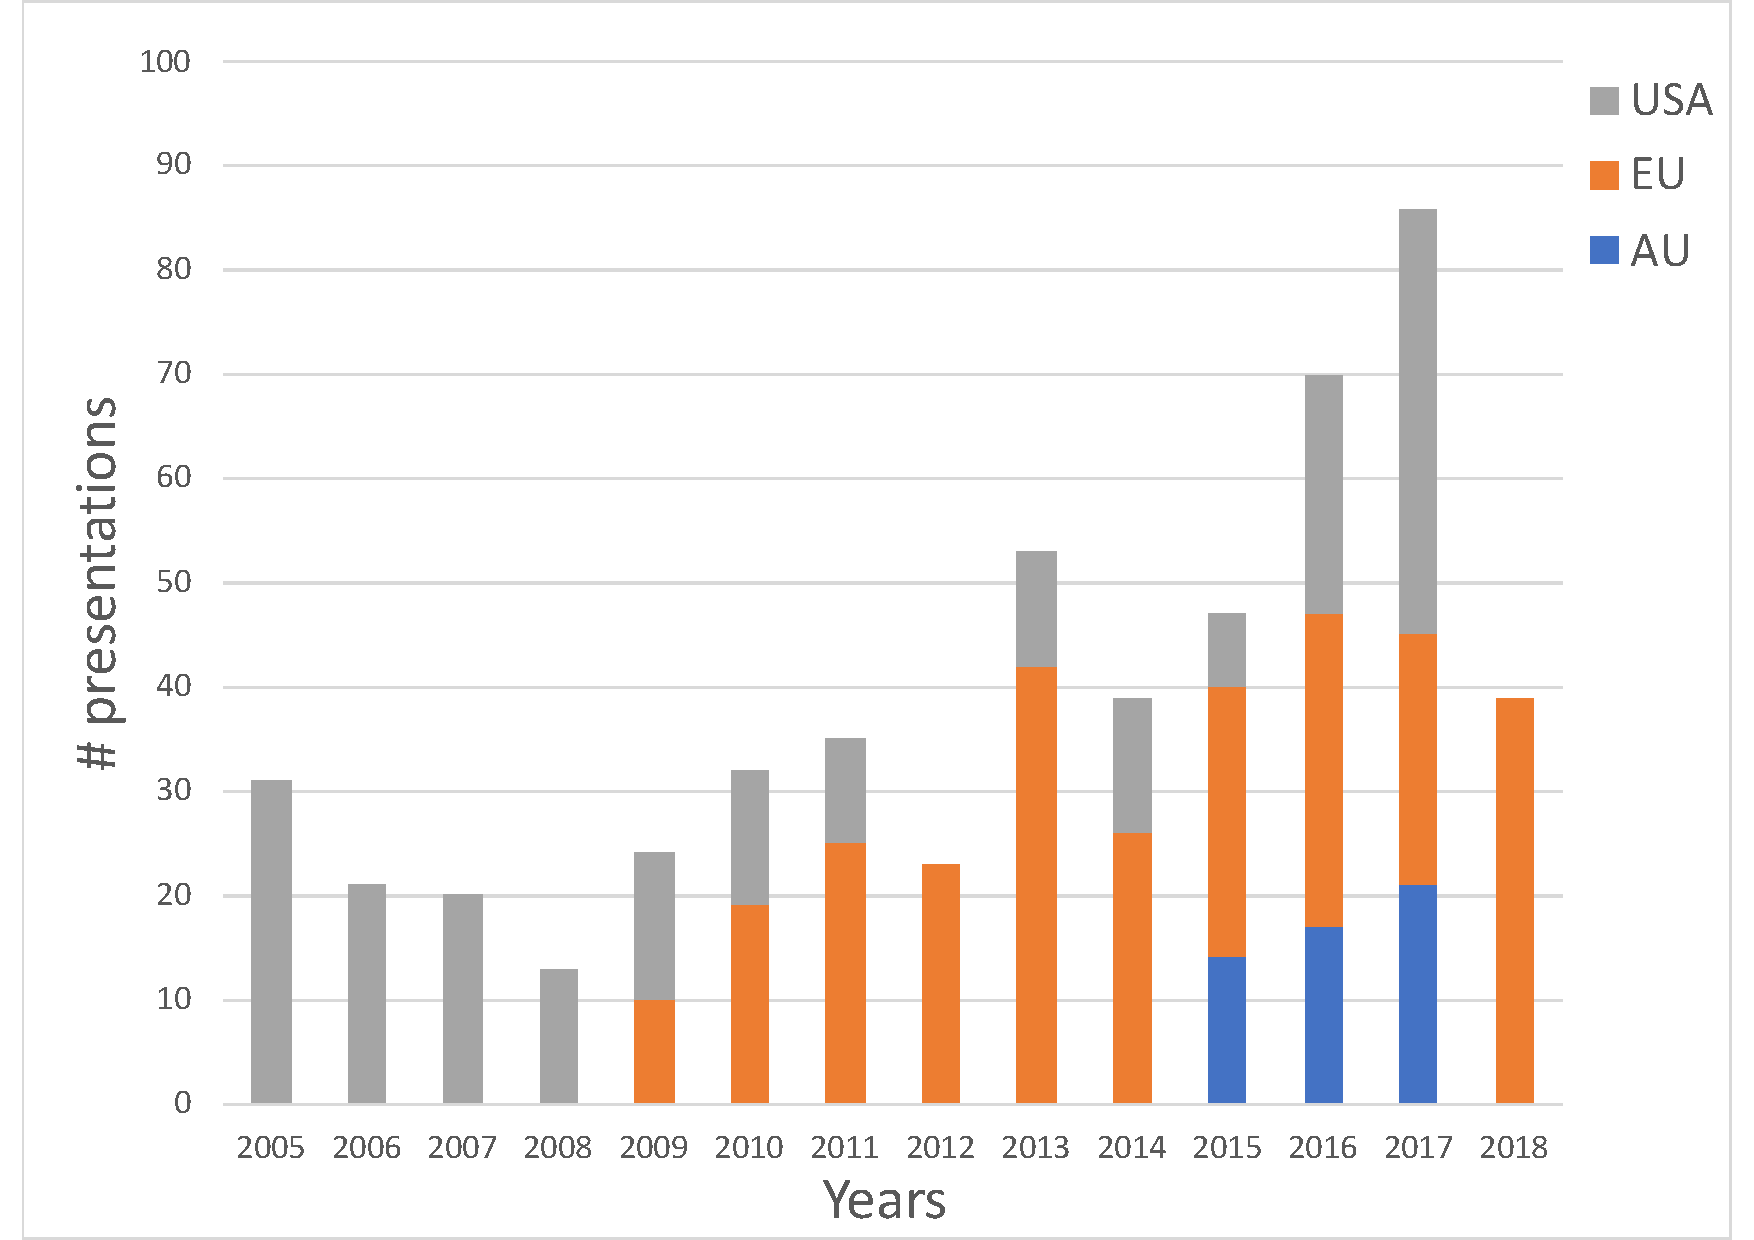
\includegraphics[width=0.7\linewidth]{graph}
	\centering
	\caption{Number of talks and papers presented at Science Gateway events in the USA, Europe and Australia increases through time.}
	\label{fig:graph}
\end{figure}


Initiated through the annual conferences, associated special issues on science gateways have been published by journals including the Journal of
Grid Computing (JGC)~\cite{jgc2012,jgc2015-29} and the Journal of Concurrency and Computation: Practice
and Experience (CCPE)~\cite{ccpe2005,ccpe2007,ccpe2011,ccpe2013, ccpe2013-28,ccpe2014-27,ccpe2015}. 
Currently the conference series in the USA, Europe, and Australia partner to organize a yearly special issue comprising some of the papers from all three events.




\section{The value of science gateways in the e-infrastructures landscape}

Science gateways are a key component of the emerging digital research environment. Researchers collaborate by using a global network of interacting digital platforms to access and share the leading-edge data and tools that are critical to their work. Gateways both facilitate, and are supported by, broader movements such as open research, open science, open source software and open data. Consequently, science gateways are valuable to a range of stakeholders: students and educators, individual researchers, research communities, research organizations and institutions, industry, governments, infrastructure providers and funding agencies.

\changedtext{Defining science gateways in terms of common characteristics and functionality assists in identifying their value to their stakeholders. Below we comment on the value of gateways regarding lowering barriers to e-infrastructures, enabling collaboration between (remote) researchers, sharing and linking infrastructure resources, driving standards and open science, and supporting teaching and new career developments.  }


\changedtext{\textbf{Lowering barriers.}}
Science gateways lower barriers by hiding the complexity of the underlying digital research infrastructure and simplifying access to best-practice tools, data and resources, thereby democratizing their usage. 
An example is CBRAIN, a web-based collaborative research platform that offers transparent access to remote data sources, distributed computing sites, and an array of processing and visualization tools for neuroimaging research~\cite{cbrain-70}. 

Some  gateways provide access to  modelling and other software and hardware resources through a single portal. Researchers do not need to spend time downloading, installing and updating software on hardware that they also maintain. 
Instead, they can use the latest optimized software on powerful remote hardware completely through the web, of which nanoHUB provides an impressive example~\cite{nanohub-33}. 

\changedtext{\textbf{Enabling collaboration.}}
Science gateways can enable collaboration and build communities through facilitated sharing of data and analyses among multidisciplinary and geographically dispersed research groups, leading to increased openness. REMEDI illustrates well  how successful collaboration was established through a science gateway: it is a collaborative community of pharmacists, nurses, researchers, vendors and others working to improve patient safety and healthcare quality through the development and exchange of infusion pump medication administration knowledge and best practices~\cite{remedi-71}.  

Researchers no longer need to be physically co-located because resources can be globally distributed, with only an internet connection needed for participation. This also enables inclusion of less advantaged researchers/institutions. 
The Sci-GaIA project has demonstrated this through its tremendous success in deploying a vast array of applications available through the African Grid Science Gateway. 
\changedtext{Building on information and communication technology investments over many years, Sci-GaIA supports today a virtual collaborative community through the African Pharmacology Science Gateway and the Community Health Portal for health professionals and patients~\cite{sci-gaia-22}. }

\changedtext{\textbf{Sharing and linking resources.} }
By sharing resources across multiple institutions, the costs of setting up and supporting research infrastructure is lowered, as each institution is no longer required to support a replica of data, compute and tools at their site. For gateways that are open source, their very building and evolution can be democratized with community members contributing in the development. 
\changedtext{Many frameworks used to build  science gateways are available on GitHub}, for example Apache Airavata~\cite{airavata}, HUBzero~\cite{hubzero-55} and  Galaxy~\cite{galaxy}, Drupal~\cite{drupal} and Django~\cite{django}.

Science gateways provide these benefits to users by performing a key role in integrating e-infrastructure layers, in particular by linking together elements that can include data storage, tools, authentication, networks, cloud and high-performance computing, and access to data resources for reuse (sometimes called ``data as infrastructure''). This integration tailors digital environments to community needs without the need for expertise in navigating the enabling information technology infrastructure that supports their work. They simplify linkage to other infrastructures, such as synchrotrons, ground-based telescopes, satellites, DNA sequencers, distributed archives and performance art studios. In some cases, the science gateway architecture supports the whole research process from hypothesis generation to results analysis, including provenance information. One example is the VRE under construction in the EVER-EST project~\cite{everest-73}, which will support handling of research objects along the complete information lifecycle in Earth science research. 

\changedtext{\textbf{Driving standards and open science.}}
Science gateways interact with the e-infrastructures landscape in multiple ways. At the broadest level, science gateways play a key role in driving standards and policy compliance, supporting initiatives including open research, open science, open source software, and open data.  Zooniverse, for instance, is a science gateway that promotes  citizen science, where anyone can be in the seat of a researcher (and define a project) or a volunteer (and perform some task in the project)~\cite{zoo-76}. 

Science gateways can also both drive standards and act as testbeds, as the increased user expectations encouraged by science gateways can drive requirements for harmonization. These standards often arise from sharing of best practice, with communities of practice addressing issues including reproducibility, sustainability, interfaces to cloud computing, workflows, integration of scientific instruments, success metrics, usability studies, scaling, mobile applications and security. 
An increasing number of international organizations address some of these issues. These include the Software Sustainability Institute; the US Research Software Sustainability Institute (URSSI) conceptualization project ``Working toward Sustainable Software for Science: Practice and Experiences''~(WSSSPE~\cite{wssspe}), the FORCE11 Software Citation Implementation Working Group~\cite{force11-39} and COS, the Center for Open Science~\cite{cio}. 
A one-week bootcamp offered by the Science Gateways Community Institute helps developers articulate the value of their work to key stakeholders and to create a strong development, operations, and sustainability plan. Working in teams, participants have the opportunity to network and establish relationships with people who are engaging in similar activities. An abridged version will be offered internationally for the first time in 2018. With diverse and constantly changing technologies available, collaboration among practitioners continues to be essential to share best practice and to avoid reinventing the wheel, helping developers to easily tailor science gateways for specific user communities.

\changedtext{\textbf{Enable cross-disciplinary research.}}
Science gateways also provide valuable resources for cross-disciplinary research, and increased interoperability across science gateways will enable more multidisciplinary research. The adoption of common interfaces and formats to build a global network of science gateways will further promote open and reproducible science, and will increase the availability and usage of existing scientific tools and data. This will lead to the emergence of a new class of scientific services such as application stores, search engines and continuous integration services. 
Science gateways are beginning to access the services of other gateways, allowing gateway developers to design interfaces and implement functionalities specific to their communities, yet use already built infrastructure as it exists elsewhere. 
For example, the Characterisation Virtual Laboratory produces and supports software that is used internationally~\cite{cvl}, and their MyTardis software is being deployed by Euro-Bioimaging in partnership with ELIXIR Finland at the Global Bioimaging head node in Turku, Finland. 
Another example is the CIPRES science gateway~\cite{Miller2012-40}, which provides an API interface to its software-as-a-service offerings, allowing others developing gateways to use those services from within their own frameworks.

Whilst some gateways already cross a number of disciplines to answer research questions, a global, decentralized network of science gateways may emerge. In this network, platforms would expose a consistent front through open specifications offering common interfaces, formats and protocols, allowing for the exchange of data, processing tools and experiments. In such a network, common web APIs such as Agave~\cite{agave-8} or CARMIN~\cite{carmin-9} could expose methods to query and manipulate data, to run data processing tools and to share experiments. Description formats such as the Common Workflow Language~\cite{cwl-10} and Boutiques~\cite{boutiques-11}, which leverage the now-mature virtual containerization systems, will represent and install processing tools consistently in multiple science gateways from a single description. At the data level, domain-specific description formats such as the Neuroimaging Data Model~\cite{nidm-12}, the Brain Imaging Data Structure~\cite{bids-13}, the Minimal Standard for Adaptive Immune Receptor Repertoires~\cite{rubelt-82,Breden-83}, or the data models provided by the International Virtual Observatory Alliance (IVOA)~\cite{ivoa-14}, will facilitate the exchange of datasets and the improvement of existing data models for new categories of scientific experiments. 
%The adoption of common interfaces and formats to build a global network of science gateways will further promote open and reproducible science, it will increase the availability and usage of existing scientific tools and data, and it will lead to the emergence of a new class of scientific services such as application stores, search engines and continuous integration services.

An important requirement for  interoperability is a common vision about how to provide the research communities with federated access to a VRE. 
Significant effort has been put in this direction by the EC-funded project AARC~\cite{aarc-50} (and the recently approved  AARC2) towards an interoperable architectural design, policy harmonization and community-driven piloting activity. Some examples of AARC-compliant e-infrastructures are the EGI CheckIn Service~\cite{aai-51}, the  INDIGO-Datacloud~\cite{indigo-52} Authentication and Authorization Infrastructure (AAI)  and the INAF Cherenkov Telescope Array (CTA) AAI, which includes the INAF-CTA Science Gateway~\cite{Costa2015-53}. The H2020 VRE4EIC project is also dedicated to definition of an interoperability framework that will enable exchange of resources among science gateways more easily~\cite{vre4eic-21}.

Related to the need for science gateway interoperability is a need for an effective discovery mechanism to assist researchers in identifying existing software that might meet their needs. Registries of science gateways and other software for research do exist, but there is no single authority for these resources at an international level. The current ecosystem is a combination of registries for individual reusable gateways \cite{alces-54, hubzero-55} that do not necessarily inter-operate, general software registries that include scientific components~\cite{github-56,openhatch-57}, funder-specific registries~\cite{canarie-58}, and registries that are limited to one, or a handful of related disciplines~\cite{iplant-59,cyverse-60}. Since there is already a proliferation of registries as described above, a federated approach is more appropriate than the creation of yet another registry. Such a federation would not only support search and discovery, but in the longer term it opens the door for dynamic creation of workflows based on publicly available components.

\changedtext{\textbf{Education and career development.}}
Science gateways also have a role in education, training researchers of the future and providing access to methods formerly only accessible to experts. Examples are CLEERhub~\cite{cleerhub-74} for Science, Technology, Engineering, and Mathematics (STEM) and STEM-–related disciplines, and Vortex Shedding, which provides a free on-line educational environment for high school and college level students to learn about physical phenomena~\cite{vortex-75}.

The majority of analyses of both specific science gateways and large e-infrastructure programs emphasize the importance of appropriate skills and training. Web technologies such as HTML5, WebGL, and JavaScript frameworks have never been so agile and fast developing as in the last five years, leveraging possibilities to utilize applications more efficiently and more effectively with increased positive user experience. 
Many of the organizations mentioned here include a focus on this crucial need of developing skills in a fast changing technology landscape. 
For example the Science Gateways Community Institute features a Workforce Development component that includes a coding institute, workshops and summer internships where students are paired with gateway developers working on real world problems. Also, Indiana University offers a graduate level course on Science Gateway Architectures \cite{course-86}. 
A key question is what skills do all researchers need, versus what will remain as specialist knowledge, particularly with regard to informatics. Where specialist skills are needed, career paths, recognition mechanisms and training opportunities are critical, as common issues emerge in integrating tools, applications, and data collections through a tailored web-based environment. 
It is also essential that scientists, researchers and students are able to learn and adopt a new set of software-related skills and methodologies, as well as learning to collaborate virtually amongst teams that are widely distributed. 
Many research communities or science gateways also provide their own programs. This is the case of the Biodiversity and Climate Change Virtual Laboratory's EcoEd program, which provides training in the use of virtual laboratories and data repositories available to ecosystem scientists and lecturers~\cite{ecoed-81}. 


\section{The impact of science gateways}

\changedtext{Science gateways have diverse goals, diverse user communities and diverse measures of success. 
But in all cases, measurement and characterization of impact is of fundamental importance.
Each science gateway measures impact differently, making it difficult to collate the various measures being used into global indicators. However, a} 
 range of ways exist to quantitatively provide evidence for the impact of individual science gateways:
\begin{itemize}
	\item number of users and individual researchers,
	\item number of laboratories and groups served,
	\item number of organizations,
	\item computing infrastructure activity (number of jobs, computing time and storage),
	\item number of  citations (to Science Gateways),
	\item number of  (enabled) publications,
	\item value of access to software,
	\item value of access to data,
	\item contingent valuation,
	\item efficiency savings, and
	\item return on investment.
\end{itemize}

\changedtext{Different science gateways (programs) utilize different combinations of measures.} Traditional metrics such as user numbers are still actively used, and some groups also use more impact-focused studies to demonstrate contingent valuation. These are often used alongside emerging measures such as software citation~\cite{force11-32}. 
It would also be useful to be able to analyse the sustainability of science gateways (beyond initial grant funding) as another measure of success.


It is difficult to make comparisons across science gateway programs due to their different structures and ways of measuring impact. For example, Nectar-funded virtual laboratories identify over 23,000 users; however, the methods used by each virtual laboratory to measure users can vary widely. In contrast, CANARIE defines users as referring to research teams or groups, rather than individual researchers. 
While the US-based XSEDE program does not fund gateways, dozens of gateways use its compute resources. 
In an Interim Project Report from 2018 \cite{xsede-85}, Table 12-1 shows gateway users varying between 10,000 and 12,000 in 2017, about four times higher than active users at the command line.  There are also many successful gateways that do not need high-end computing, for example, the vast majority of the more than a million nanoHUB users~\cite{nanohub-33}, for which such metrics would not be appropriate.

Part of the evidence for the value of science gateways comes from work highlighting the importance of e-infrastructures, such as Mayernik, Hart, Maull and Weber's work~\cite{Mayernik-34}. They note the increasing recognition that ``traditional assessments of research impact have missed broad swaths of important activities, including the benefits associated with the collection, management and preservation of digital resources, such as data and software, and the provision of research facilities and services, such as computational facilities and observational platforms''. 
Metrics for quantitatively measuring the impacts of analytical tools over data are now beginning to emerge, and can contribute to the valuation of science gateways. Beagrie and Houghton's work on the European Molecular Biology Laboratory  and European Bioinformatics Institute (EMBL-EBI) assessed the value and impact of the EMBL-EBI by identifying four valuation levels: access (use) value, contingent valuation, efficiency savings, and return on investment~\cite{Beagrie2016-35}. 
This was applied to a range of EMBL-EBI services, including both data access and analytical services over the data –- one of very few studies examining the latter. In 2017, Nectar commissioned Victoria University to apply Beagrie and Houghton's methodology to evaluate the economic impact of virtual laboratories. The report measures the economic benefits created in five different ways. For all three of the virtual laboratories, each measure shows that the economic benefit is greater than the investment required.  Taking a long term perspective, the research enabled by the virtual laboratories generates substantial returns compared to their costs~\cite{nectar-80}.

The need for science gateways is also being demonstrated through increasing acknowledgment of the critical role of software in research. A 2009 survey by Hannay, MacLeod, Singer, Langtangen, Pfahl and Wilson with 2,000 responses showed that 84\% of researchers view the development of software as ``important or very important for their own research''~\cite{Hannay2009-36}. The USA's National Science Foundation's research software vision identifies software as ``directly responsible for increased scientific productivity and significant enhancement of researchers' capabilities''~\cite{nsf-si-17}. 
Further, in 2014 a survey funded by the National Science Foundation sent to NSF-funded principal investigators and Chief Information Officers and Chief Technology Officers at US academic institutions resulted in  5,000 respondents. In total 88\% indicated a reliance on science gateway-like interfaces to conduct their work and 57\% were themselves involved in some capacity in the creation of these~\cite{Lawrence2015-37}.

A recent study applied a similar methodology to the Industrial Ecology Virtual Laboratory (IELab), a high-performance computing lab used for compiling large-scale, high-resolution, enviro-socio-economic accounts for the purpose of conducting integrated sustainability assessment project~\cite{Wiedmann2017-38}. 
Wiedmann's analysis of 30 IELab publications that were published in either peer-reviewed journal papers or in the form of conference proceedings, concluded that two-thirds of the studies would not have been possible without IELab, and a further 16\% would have required considerable extra resources to complete. 
This type of contingent valuation could also be inferred from other metrics, such as the emerging emphasis on software citations, an area where organisations such as the FORCE11 Software Citation Implementation Working Group~\cite{force11-39} is undertaking significant work. For example, the CIPRES Science Gateway (for phylogenetic research) has enabled 3,000 publications since 2010. Without this science gateway, many users would not have undertaken this type of research, instead needing to set up their own clusters, and install, maintain and optimize the many pieces of software offered via CIPRES~\cite{Miller2012-40}. 

\section{Conclusion: opportunities for science gateways}

Science gateways have been a valuable addition to the digital infrastructure landscape, facilitating more efficient, open, reproducible research. The many science gateway initiatives available provide abundant opportunities for reflection, identification of best practice and analysis of beneficial ways forward. Some of the key areas in which continued collaboration may advance the field include:
\begin{itemize}
	\item Technical solutions for the development of science gateways, including interoperability, standards, software registries, and data management.
	\item Best practices and policies for the valuation of science gateways, including incentives for open science, reproducibility, data and software citation.
	\item Sustainability models for the maintenance, development, and exploitation of science gateways, including development of skills, training, career paths and funding.
\end{itemize}

For example, developing interoperability across science gateways is key to a successful conduct of collaborative data- and compute-intensive research, to enable open data and reuse of methods across domains and applications. 
The adoption of common interfaces and formats to build a global network of science gateways will create a new class of scientific services that will increase accessibility to tools and data,  further promoting open and reproducible science. 


In conclusion, it is important that the field of science gateways continues to evolve, increasing interoperability to enable more multidisciplinary research, increasing collaboration and sharing mechanisms, to facilitate more efficient, open, and reproducible research. 
Appropriately skilled users and developers also need to be trained in tandem with this software infrastructure, to ensure the maximum value of the infrastructure is realized and to further facilitate increased research impacts. 
The ongoing investment in national and international programs, in tandem with community and disciplinary initiatives, are facilitating the development of many communities of practice to address these issues, including ways to demonstrate the value of contributions of individuals, science gateways, and national and international programs to this field. Increasing coordination across these varied initiatives will continue to improve identification of best practice and development of policies and standards, enhancing the ability of science gateways to increase the impact of research.


\section*{References}

\bibliography{mybibfile}

\section*{Author contributions}
All authors participated in the conception and writing of the paper and also approved the manuscript.

\section*{Funding sources} 
SG is funded via SGCI, NSF Award Number ACI-1547611, via US Research Software Sustainability Institute (URSSI) conceptualization, NSF Award Number ACI-1743188 and via the Center for Research Computing at the University of Notre Dame as well as HUBzero.
BC is a member of the iReceptor Project, which is supported by funding from CANARIE, the Canada Foundation for Innovation, and the BC Knowledge Development Fund.
NCH is supported by EPSRC, BBSRC and ESRC Grant EP/N006410/1 for the UK Software Sustainability Institute and has received funding from Jisc in the last five years.
KJ is funded by the VRE4EIC project, which has received funding from the European Union’s Horizon 2020 research and innovation programme under grant agreement No 676247.


\section*{Declaration of interest}
MB is employed by Nectar, and co-convenor of the ICSG and IWSG-A.
BC is a member of the CANARIE Software Technology Advisory Committee.
HG is a member of the project team for the H2020-funded EVER-EST VRE initiative, co-chair of the RDA VRE interest group and also a member of the RDA Technical Advisory Board (TAB).
SDO is part of SGCI, was part of the SCI-BUS project funded by the FP7 e-infrastructures program, and currently acts as European Liaison for HUBzero.
NCH is PI of the Software Sustainability Institute and a member of the US Research Software Sustainability Institute (URSSI) Advisory Committee.
DSK and NCH are co-chairs of the FORCE11 Software Citation Implementation Working Group.
DSK and SG are co-PIs of the US Research Software Sustainability Institute (URSSI) conceptualization.
SG is part of SGCI, co-chair of the RDA VRE interest group, chair of the IEEE Technical Area on Science Gateways and PI of “Evaluation of HUBzero® as a Platform to Service a Diverse Set of Scientific Communities”.
LW is a co-chair of the RDA VRE interest group and has received funding from Nectar and the Australian National Data Service to develop the Virtual Geophysics Laboratory.

\clearpage

\begin{landscape}% Landscape page
\begin{center}

\setlength\LTcapwidth{\linewidth}

\begin{longtable}[c]{lllll}

\caption{Overview of science gateways events showing year, number of presentations (talks and papers), event name, location, and links to the proceedings and/or program.}
\label{tab:table} \\


	\hline 
	\multicolumn{1}{l}{Year} &
	\multicolumn{1}{l}{\#} &
	\multicolumn{1}{l}{Event} &
	\multicolumn{1}{l}{Location} &
	\multicolumn{1}{l}{Proceedings and Agendas} 
	\\ \hline
	\endfirsthead


	\multicolumn{5}{l}{\tablename\ \thetable{} --
		continued from previous page} \\
\hline
\endhead
	
	\hline
	\endlastfoot

2005 & 15 & ScienceGgateways\footnote{with Global Grid Forum} & Chicago,  US-IL & 
{\tiny \url{https://onlinelibrary.wiley.com/doi/pdf/10.1002/cpe.1098}} \\

2005 & 16 & GCE  & Seattle,  US-WA &
{\tiny \url{http://onlinelibrary.wiley.com/doi/10.1002/cpe.1258/full}} \\

2006 & 21 & GCE & Tampa,  US-FL & 
{\tiny \url{http://www.cogkit.org/GCE06}} \\

2007 & 20 & GCE  & Reno,  US-NV & 
{\tiny \url{https://www.researchgate.net/publication/}}
\\ &&&& 
{\tiny \url{259366865_International_Workshop_on_Grid_Computing_Environments_2007_in_Conjunction_with_SC07}} \\

2008 & 13 & GCE  & Austin,  US-TX &
{\tiny \url{ https://ieeexplore.ieee.org/xpl/mostRecentIssue.jsp?punumber=4729055}} \\

2009 & 14 & GCE  & Portland,  US-OR & 
{\tiny \url{
		http://dblp.uni-trier.de/db/conf/sc/gce2009.html}} \\

2009 & 18 & IWPLS\footnote{International Workshop on Portals for Life Sciences}  & Edinburg,  UK &
{\tiny \url{ http://ceur-ws.org/Vol-513/}}  \\

2010 & 13 & GCE  & New Orleans,  US-LA &
{\tiny \url{  http://www.proceedings.com/10226.html}} \\

2010 & 19 & IWSG  & Catania,  IT &
{\tiny \url{  http://agenda.ct.infn.it/event/347/}} \\

2011 & 10 & GCE & Seattle,  US-WA & 
{\tiny \url{ https://dl.acm.org/citation.cfm?id=2110486}} \\

2011 & 25 & IWSG-Life & London,  UK &
{\tiny \url{ https://sites.google.com/a/staff.westminster.ac.uk/iwsg-life2011}}
\\&&&&
{\tiny \url{ http://ceur-ws.org/Vol-819/ }} \\

2012 & 23 & IWSG-Life & Amsterdam,  NL &
{\tiny \url{  https://sites.google.com/site/iwsglife2012}}
\\ &&&& 
{\tiny \url{ http://ebooks.iospress.nl/volume/healthgrid-applications-and-technologies-meet-science-gateways-for-life-sciences }} \\

2012 & n.a. & GCE &    & not held this year
\\

2013 & 11 & SGCI Workshop\footnote{While in conceptualization phase} & Indianapolis,  US-IN & 
{\tiny \url{ https://ieeexplore.ieee.org/xpl/mostRecentIssue.jsp?punumber=6689497 }} \\

2013 & 42 & IWSG  & Zurich,  CH &
{\tiny \url{  https://en.xing-events.com/iwsg2013.html }} 
\\ &&&&
{\tiny \url{http://ceur-ws.org/Vol-993/}} \\

2014 & 13 & GCE  & New Orleans,  US-LA &
{\tiny \url{  https://dl.acm.org/citation.cfm?id=2690887 }} \\

2014 & 26 & IWSG  & Dublin,  IE &
{\tiny \url{  https://sites.google.com/a/my.westminster.ac.uk/iwsg2014/home/dates }} 
\\ &&&&
{\tiny \url{ https://ieeexplore.ieee.org/xpl/mostRecentIssue.jsp?punumber=6881322 }}\\

2015 & 16 & GCE & Boulder,  US-CO &
{\tiny \url{ https://onlinelibrary.wiley.com/doi/epdf/10.1002/cpe.3743 }} \\

2015 & 26 & IWSG & Budapest,  HU&
{\tiny \url{  https://ieeexplore.ieee.org/xpl/mostRecentIssue.jsp?punumber=7217893 }}\\

2015 & 14 & IWSG-A & Brisbane, AU & 
{\tiny \url{ https://sites.google.com/site/iwsglife/about-iwsg-a/iwsg-a-2015}} \\

2016 & 34 & Gateways & San Diego,  US-CA & {\tiny \url{ https://sciencegateways.org/gateways2016/program }}
\\&&&&
{\tiny \url{  https://gateways2016.figshare.com}} \\

2016 & 30 & IWSG & Rome,  IT & 
{\tiny \url{ https://sites.google.com/a/nd.edu/iwsg2016/home http://ceur-ws.org/Vol-1871}} \\

2016 & 17 & IWSG-A & Melbourne, AU & 
{\tiny \url{ https://sites.google.com/site/iwsglife/about-iwsg-a/iwsg-a-2016}} \\

2017 & 41 & Gateways & Ann Arbor,  US-MI & 
{\tiny \url{ https://sciencegateways.org/web/gateways2017/program}}
\\&&&&
{\tiny \url{  https://gateways2017.figshare.com }}  \\

2017 & 24 & IWSG & Poznan,  PO & 
{\tiny \url{ http://iwsg2017.psnc.pl/programme}} \\

2017 & 21 & IWSG-A & Brisbane, AU & 
{\tiny \url{ http://iwsg-life.org/site/iwsglife/about-iwsg-a }} \\

2018 &	39 &	IWSG &	Edinburgh, UK &	
{\tiny \url{ https://sites.google.com/a/nd.edu/iwsg2018}}	

\end{longtable}
	


\end{center}
\end{landscape}% Landscape page

\end{document}